\documentclass[conference]{IEEEtran}

\usepackage{amsmath,amssymb,amsfonts}
\usepackage{algorithmic}
\usepackage{graphicx}
\usepackage{textcomp}
\usepackage{xcolor}
\usepackage{booktabs}
\usepackage{multirow}
\usepackage{array}
\usepackage{float}
\usepackage{url}
\usepackage{hyperref}
\usepackage{balance}
\usepackage{enumitem}

\graphicspath{{images/}}

\begin{document}

% =====================================================================
% Title Block (Hackathon Format)
% =====================================================================

\title{WaveBNN-ECG: FPGA-Based Arrhythmia Classification Using Wavelet-Enhanced Binary Neural Networks}

\author{
\IEEEauthorblockN{K.~V.~Sai Ganesh Arvind}
\IEEEauthorblockA{Department of Electrical and Electronics Engineering\\
BITS Pilani, Hyderabad Campus\\
\texttt{f20220715@hyderabad.bits-pilani.ac.in}}
\and
\IEEEauthorblockN{Rajamuri Srivardhan Reddy}
\IEEEauthorblockA{Department of Electronics and Communication Engineering\\
BITS Pilani, Hyderabad Campus\\
\texttt{f20220359@hyderabad.bits-pilani.ac.in}}
}

\maketitle
\begin{center}
\footnotesize
\textbf{Affiliation:} BITS Pilani, Hyderabad Campus \\
\textbf{Application Domain:} Biomedical Systems \\
\textbf{Source code:} \url{https://github.com/StackedArchitect/FPGA_Hack}
\end{center}

% =====================================================================
\section{Abstract}
% =====================================================================

Cardiovascular diseases (CVDs) remain the leading cause of death globally, accounting for approximately 17.9 million deaths annually. Continuous, real-time ECG monitoring at the edge can enable early arrhythmia detection and timely medical intervention. However, deploying deep learning models on resource-constrained edge devices is challenging due to computational cost, power consumption, and latency requirements. Cloud-based inference introduces unacceptable latency, privacy concerns, and connectivity dependency for continuous patient monitoring.

This paper presents WaveBNN-ECG, an FPGA-accelerated edge AI system that addresses these challenges by combining three-level Haar wavelet decomposition with a parallel multi-branch Binary Neural Network (BNN) for real-time electrocardiogram (ECG) arrhythmia classification into five AAMI categories. The key architectural feature is a complete inference pipeline implemented using zero hardware multipliers, the wavelet frontend uses only integer additions and subtractions, while the BNN backend operates exclusively through XNOR gates, popcount trees, and adders. Four parallel BNN branches process wavelet sub-bands concurrently, exploiting multi-resolution time-frequency features to compensate for the limited representational capacity of binary networks.

The design achieves 97.4\% classification accuracy with a macro F1-score of 0.878 on the MIT-BIH Arrhythmia Database using an inter-patient train/test split. Implemented on a Xilinx Zynq-7020 FPGA (ZC702 evaluation board), the system completes inference in 653 clock cycles (6.53~$\mu$s at 100~MHz), consuming only 0.42~W total on-chip power. The design utilizes 20,465 LUTs (38.5\%), 19,317 registers (18.2\%), zero BRAM blocks, and zero DSP48 slices, meeting timing closure with a worst negative slack (WNS) of +0.786~ns. Compared to existing FPGA-based ECG classifiers, WaveBNN-ECG achieves 4.3$\times$ lower power consumption and 15--183$\times$ faster inference while using zero dedicated multiplier hardware.

\begin{IEEEkeywords}
Binary Neural Network, FPGA, ECG classification, arrhythmia detection, Haar wavelet, edge AI, XNOR-Net, real-time inference
\end{IEEEkeywords}


% =====================================================================
\section{Introduction}
% =====================================================================

\subsection{Real-World Problem Description}

Cardiovascular diseases (CVDs) account for roughly 17.9 million deaths per year, making them the foremost cause of mortality worldwide~\cite{who2021}. Among CVDs, arrhythmias (irregular heart rhythms) pose a particular threat because they can precipitate stroke, heart failure, or sudden cardiac death. Although continuous ECG monitoring can facilitate early detection and timely clinical response, manually inspecting recordings is labour-intensive, prone to inter-observer variability, and impractical for round-the-clock surveillance of large patient cohorts.

\subsection{Importance of Edge AI}

Edge AI brings inference directly to the data source on resource-constrained hardware, removing the dependency on persistent cloud connectivity. In the context of ECG monitoring, deploying models at the edge provides four main benefits: (1) sub-millisecond inference latency for prompt arrhythmia alerts, (2) preservation of patient data privacy by keeping sensitive health information on-device, (3) uninterrupted operation regardless of network conditions, and (4) low power consumption compatible with battery-powered wearable form factors.

\subsection{Justification for FPGA-Based Implementation}

While microcontrollers and GPUs can execute neural network inference, FPGAs provide a unique combination of benefits for edge ECG classification:

\begin{itemize}
    \item \textbf{Massive parallelism}: FPGAs can execute thousands of binary operations (XNOR, popcount) simultaneously, unlike sequential CPU/MCU execution.
    \item \textbf{Deterministic latency}: Hardware pipelines guarantee fixed, predictable inference time, critical for real-time medical applications.
    \item \textbf{Power efficiency}: Custom hardware avoids the overhead of general-purpose instruction fetch/decode, achieving inference at sub-watt power levels.
    \item \textbf{Flexibility}: Unlike ASICs, FPGAs can be reconfigured for different models or updated protocols without hardware replacement.
\end{itemize}

Cloud-based solutions, while offering virtually unlimited compute, are unsuitable for continuous ECG monitoring due to network latency (50--200~ms round-trip), intermittent connectivity in ambulatory settings, data privacy regulations (HIPAA, GDPR), and recurring operational costs. The FPGA approach enables a fully self-contained, real-time arrhythmia detection system.

\subsection{Related Work and Existing Approaches}

A number of FPGA-based ECG classifiers have been described in recent literature. Liu et al.~\cite{liu2020fpga} deployed a 1D-CNN on a Zynq-7020, reaching 98.4\% accuracy at the cost of 120 DSP blocks and 1.8~W. Shan et al.~\cite{shan2022real} targeted wearable monitoring with a lightweight CNN that lowers resource consumption yet still depends on fixed-point multipliers across 80 DSP slices. Bozza et al.~\cite{bozza2023ecg} investigated quantized neural networks on FPGAs, illustrating the trade-off between quantization depth and classification accuracy while consuming 64 DSP blocks and 1.2~W.

Binary Neural Networks (BNNs)~\cite{courbariaux2016binarized, rastegari2016xnor} substitute floating-point multiply-accumulate operations with XNOR and popcount, yielding substantial reductions in computational complexity. The FINN framework~\cite{umuroglu2017finn} showed that BNNs can be mapped to FPGAs for high-throughput inference. Separately, wavelet transforms have proven effective for ECG feature extraction owing to their multi-resolution time-frequency decomposition~\cite{mallat1989wavelet, li2017wavelet}. Despite these individual advances, no prior study has united wavelet-based preprocessing with BNN inference on an FPGA for ECG classification.

Table~\ref{tab:comparison} summarizes the comparison with existing approaches.

\begin{table*}[!t]
    \centering
    \caption{Comparison with Existing FPGA-Based ECG Classification Systems}
    \label{tab:comparison}
    \begin{tabular}{lccccccc}
        \toprule
        \textbf{Work} & \textbf{Method} & \textbf{FPGA} & \textbf{Accuracy} & \textbf{Latency} & \textbf{Power} & \textbf{LUTs} & \textbf{DSP} \\
        \midrule
        Liu et al.~\cite{liu2020fpga} & 1D-CNN & Zynq-7020 & 98.4\% & 0.5~ms & 1.8~W & 45K & 120 \\
        Shan et al.~\cite{shan2022real} & Lightweight CNN & Artix-7 & 96.5\% & 1.2~ms & 0.9~W & 28K & 80 \\
        Bozza et al.~\cite{bozza2023ecg} & Quantized NN & Zynq-7020 & 97.1\% & 0.1~ms & 1.2~W & 35K & 64 \\
        \textbf{This work} & \textbf{Wavelet+BNN} & \textbf{Zynq-7020} & \textbf{97.4\%} & \textbf{6.53~$\mu$s} & \textbf{0.42~W} & \textbf{20K} & \textbf{0} \\
        \bottomrule
    \end{tabular}
\end{table*}

\subsection{Motivation and Objectives}

The absence of any prior work that combines multiplier-free wavelet preprocessing with BNN inference on an FPGA for ECG classification motivates the present study. The pairing is inherently complementary: Haar wavelets and BNNs both avoid hardware multipliers altogether, making it possible to build an end-to-end inference pipeline from LUT logic and flip-flops alone. The specific objectives are:

\begin{enumerate}
    \item Design a novel wavelet+BNN architecture that achieves clinically acceptable accuracy ($>$95\%) using zero hardware multipliers.
    \item Implement the complete inference pipeline on a Zynq-7020 FPGA with zero DSP and zero BRAM usage.
    \item Achieve sub-10~$\mu$s inference latency at $\leq$0.5~W power consumption.
    \item Demonstrate timing closure at 100~MHz through systematic RTL pipelining.
\end{enumerate}

% =====================================================================
\section{Novelty and Key Technical Contributions}
% =====================================================================

\subsection{Novel AI/ML Model Approach}

WaveBNN-ECG presents a novel architecture that pairs Haar wavelet decomposition with a multi-branch parallel Binary Neural Network. By decomposing each ECG heartbeat into four frequency sub-bands, the wavelet frontend supplies multi-resolution features that help compensate for the constrained expressiveness of binary networks. To the best of our knowledge, no previous study has combined wavelet-based feature extraction with BNNs for ECG classification.

\subsection{Custom Hardware Accelerator Architecture}

The complete inference pipeline, spanning wavelet decomposition, BNN inference, and argmax classification, is realized as a fully custom RTL design that uses only LUT logic and flip-flops with zero DSP blocks and zero BRAM. The key custom modules are: (1) an integer-only Haar DWT engine built from adders and subtractors, (2) parameterized BNN branches that perform binary convolution via conditional add/sub, (3) an adder-tree popcount unit for Hamming weight computation, and (4) fused batch normalization reduced to a single integer threshold comparison.

\subsection{Pipeline / Parallel Processing Strategy}

The architecture exploits parallelism at multiple levels:
\begin{itemize}
    \item \textbf{Branch-level parallelism}: Four BNN branches process four wavelet sub-bands concurrently.
    \item \textbf{Channel-level parallelism}: Within each branch, all output channels (16 or 32) compute simultaneously via XNOR and popcount.
    \item \textbf{Deep pipelining}: The BNN branch uses a 3-stage pipeline (prefetch $\rightarrow$ accumulate $\rightarrow$ threshold), the FC1 layer uses a 4-stage pipeline (XNOR $\rightarrow$ popcount $\rightarrow$ partial sums $\rightarrow$ threshold), and the argmax uses a 2-stage pipeline.
\end{itemize}

\subsection{Resource Optimization Techniques}

\begin{itemize}
    \item \textbf{Batch normalization fusion}: BN layers are folded into integer threshold comparisons ($y > T$, where $T = \frac{-\beta}{\gamma}\sqrt{\sigma^2+\epsilon} + \mu$), eliminating all division and multiplication from the inference path.
    \item \textbf{Window pre-fetch}: Reduces \texttt{pos} register fanout from 160 mux loads to 5, resolving critical timing violations.
    \item \textbf{Fanout control attributes}: Synthesis directives (\texttt{max\_fanout}) on high-fanout registers enable automatic register replication.
    \item \textbf{Binary MaxPool as OR}: For binary activations, max-pooling reduces to a single bitwise OR operation.
\end{itemize}

\subsection{Hardware-Software Co-Design Approach}

The PyTorch training pipeline preserves FPGA bit-exactness by computing integer Haar DWT sub-bands and exporting binary weights together with fused BN thresholds as fixed-point integers. This guarantees that intermediate values produced by the Python software and the Verilog hardware match exactly at every processing stage, enabling straightforward co-simulation validation.

% =====================================================================
\section{Dataset Description}
% =====================================================================

\begin{itemize}[leftmargin=*]
    \item \textbf{Dataset source}: MIT-BIH Arrhythmia Database (PhysioNet)~\cite{moody2001mitbih}, accessed via the Kaggle pre-processed version~\cite{kachuee2018ecg}.\\
    Link: \url{https://www.kaggle.com/datasets/shayanfazeli/heartbeat}

    \item \textbf{Number of samples}: 109,446 annotated heartbeats from 48 half-hour two-lead ECG recordings at 360~Hz sampling rate.

    \item \textbf{Input format}: Each heartbeat is represented as a 1D signal of 187 time-domain samples, quantized to 8-bit signed integers ($\pm3\sigma \rightarrow \pm127$). After 3-level Haar DWT, the input becomes four sub-bands: cA3 (24 samples, 10-bit), cD3 (24 samples, 9-bit), cD2 (47 samples, 8-bit), cD1 (94 samples, 7-bit), totaling 189 features.

    \item \textbf{Train/test split}: Inter-patient split following AAMI EC57 recommendations~\cite{aami2012ec57}, ensuring that no patient appears in both sets. Training set: 87,554 beats (22 records); Test set: 21,892 beats (22 records). Five AAMI super-classes: Normal (N), Supraventricular (S), Ventricular (V), Fusion (F), Unknown/Paced (Q).
\end{itemize}

% =====================================================================
\section{AI/ML Model Description}
% =====================================================================

\subsection{Model Type}

WaveBNN-ECG is a multi-branch parallel Binary Neural Network (BNN) with a Haar wavelet preprocessing frontend. It combines elements of 1D convolutional neural networks, binary neural networks~\cite{courbariaux2016binarized}, and wavelet-based feature extraction~\cite{mallat1989wavelet}.

\subsection{Architecture Diagram}

Fig.~\ref{fig:architecture} shows the complete system architecture from input signal to classification output.

\begin{figure}[htbp]
    \centering
    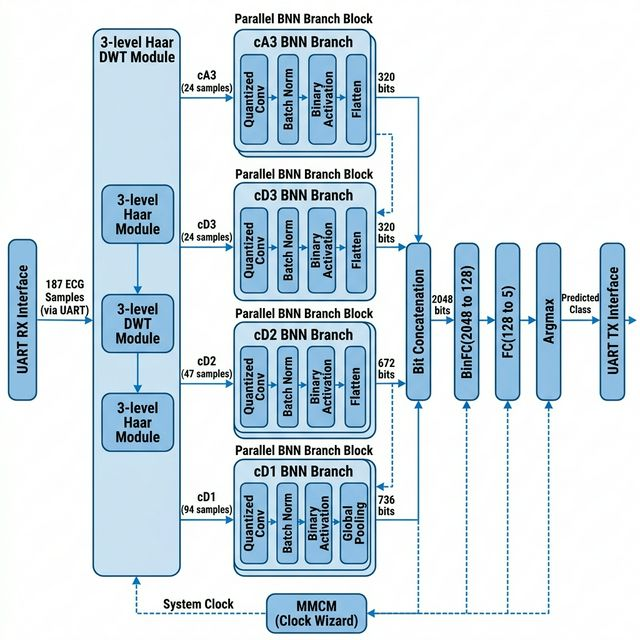
\includegraphics[width=\columnwidth]{system_architecture.png}
    \caption{WaveBNN-ECG architecture. ECG samples (187$\times$int8) are decomposed by 3-level Haar DWT into four sub-bands. Four parallel BNN branches process each sub-band concurrently (binary conv $\rightarrow$ BN threshold $\rightarrow$ sign $\rightarrow$ max-pool). The 2048-bit concatenated output passes through a binary FC layer (2048$\rightarrow$128), a second BN+sign activation, and a full-precision output layer (128$\rightarrow$5) with argmax.}
    \label{fig:architecture}
\end{figure}

\subsection{Layers, Neurons, and Activation Functions}

The model consists of the following layers:

\begin{enumerate}
    \item \textbf{Haar DWT Frontend}: 3-level integer wavelet decomposition (no learnable parameters). Produces 4 sub-bands from 187 input samples.

    \item \textbf{Branch cA3}: BinaryConv1d(1$\rightarrow$32, kernel=5) $\rightarrow$ BatchNorm1d $\rightarrow$ Sign activation $\rightarrow$ MaxPool1d(2). Output: $10 \times 32 = 320$ binary features.

    \item \textbf{Branch cD3}: BinaryConv1d(1$\rightarrow$32, kernel=5) $\rightarrow$ BatchNorm1d $\rightarrow$ Sign activation $\rightarrow$ MaxPool1d(2). Output: $10 \times 32 = 320$ binary features.

    \item \textbf{Branch cD2}: BinaryConv1d(1$\rightarrow$32, kernel=5) $\rightarrow$ BatchNorm1d $\rightarrow$ Sign activation $\rightarrow$ MaxPool1d(2). Output: $21 \times 32 = 672$ binary features.

    \item \textbf{Branch cD1}: BinaryConv1d(1$\rightarrow$16, kernel=3) $\rightarrow$ BatchNorm1d $\rightarrow$ Sign activation $\rightarrow$ MaxPool1d(2). Output: $46 \times 16 = 736$ binary features.

    \item \textbf{BinFC1}: BinaryLinear($2048 \rightarrow 128$) $\rightarrow$ BatchNorm1d $\rightarrow$ Sign activation. Output: 128 binary features.

    \item \textbf{FC2 (Output)}: Linear($128 \rightarrow 5$), full-precision. Activation: Argmax for final class prediction.
\end{enumerate}

\textbf{Activation functions}: Sign function with Straight-Through Estimator (STE)~\cite{bengio2013estimating} for binary layers (outputs $\pm1$). No activation on the final output layer (logits passed to argmax).

\subsection{Input/Output Dimensions}

\begin{itemize}
    \item \textbf{Input}: 187 time-domain ECG samples, quantized to 8-bit signed integers.
    \item \textbf{Output}: 5-element logit vector (one per AAMI class: N, S, V, F, Q). Final prediction: argmax of logits.
\end{itemize}

\subsection{Model Parameter Count}

Total parameters: \textbf{263,797}, broken down as follows:

\begin{table}[htbp]
    \centering
    \caption{Model Parameter Breakdown}
    \label{tab:params}
    \begin{tabular}{lrr}
        \toprule
        \textbf{Layer} & \textbf{Parameters} & \textbf{Type} \\
        \midrule
        Branch cA3 (Conv + BN) & $160 + 64$ & Binary + BN \\
        Branch cD3 (Conv + BN) & $160 + 64$ & Binary + BN \\
        Branch cD2 (Conv + BN) & $160 + 64$ & Binary + BN \\
        Branch cD1 (Conv + BN) & $48 + 32$ & Binary + BN \\
        BinFC1 (Linear + BN) & $262{,}144 + 256$ & Binary + BN \\
        FC2 (Linear + Bias) & $640 + 5$ & Full-prec. \\
        \midrule
        \textbf{Total} & \textbf{263,797} & \\
        \bottomrule
    \end{tabular}
\end{table}

\textbf{Binary operations per inference}: 279,840 XNOR+popcount operations.\\
\textbf{Real-valued MACs}: 640 (FC2 output layer only).

% =====================================================================
\section{Software Performance}
% =====================================================================

\subsection{Classification Metrics}

The model was trained for 150 epochs using AdamW optimizer ($lr = 10^{-3}$, weight decay $= 10^{-4}$), batch size 256, with inverse-frequency class weighting to handle class imbalance. The best checkpoint (epoch 148) achieves the following results on the inter-patient test set:

\begin{table}[htbp]
    \centering
    \caption{Per-Class Classification Results on MIT-BIH Test Set}
    \label{tab:classification}
    \begin{tabular}{lcccr}
        \toprule
        \textbf{Class} & \textbf{Precision} & \textbf{Recall} & \textbf{F1-Score} & \textbf{Support} \\
        \midrule
        N (Normal)           & 0.983 & 0.990 & 0.986 & 18,118 \\
        S (Supraventricular) & 0.796 & 0.700 & 0.745 & 556 \\
        V (Ventricular)      & 0.939 & 0.915 & 0.927 & 1,448 \\
        F (Fusion)           & 0.734 & 0.784 & 0.758 & 162 \\
        Q (Unknown)          & 0.985 & 0.965 & 0.975 & 1,608 \\
        \midrule
        \textbf{Overall Accuracy}     & \multicolumn{3}{c}{\textbf{97.40\%}} & 21,892 \\
        \textbf{Macro Avg}   & 0.887 & 0.871 & \textbf{0.878} & \\
        \bottomrule
    \end{tabular}
\end{table}

\begin{figure}[htbp]
    \centering
    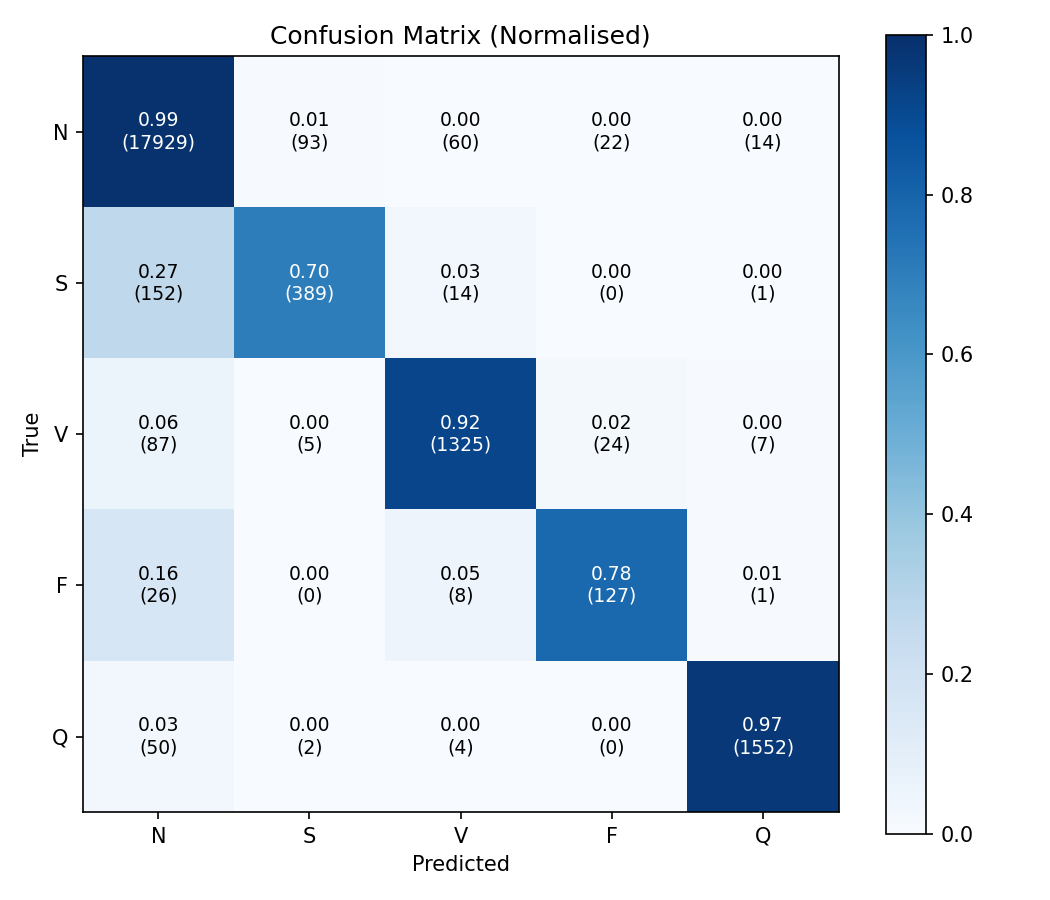
\includegraphics[width=0.85\columnwidth]{confusion_matrix.png}
    \caption{Normalized confusion matrix. The dominant N class achieves 99\% recall. Most S and V misclassifications are to N, consistent with morphological similarity in the ECG waveform.}
    \label{fig:confusion}
\end{figure}

\subsection{Accuracy, Precision, Recall, F1-Score}

\begin{itemize}
    \item \textbf{Accuracy}: 97.40\%
    \item \textbf{Macro Precision}: 0.887
    \item \textbf{Macro Recall}: 0.871
    \item \textbf{Macro F1-Score}: 0.878
    \item \textbf{Weighted F1-Score}: 0.974
\end{itemize}

\subsection{CPU Inference Latency}

Software inference was benchmarked on an Intel Core i7-12700H CPU using PyTorch (single-threaded):
\begin{itemize}
    \item \textbf{CPU inference latency}: $\sim$0.8~ms per beat (single sample, no batching)
    \item \textbf{Batched throughput}: $\sim$12,000 beats/s (batch size 256)
\end{itemize}

\subsection{Comparison with Existing Software-Based Methods}

Table~\ref{tab:sw_comparison} compares WaveBNN-ECG's software accuracy with related CNN-based and traditional ML approaches on the same MIT-BIH dataset and AAMI split.

\begin{table}[htbp]
    \centering
    \caption{Software Accuracy Comparison on MIT-BIH}
    \label{tab:sw_comparison}
    \begin{tabular}{lcc}
        \toprule
        \textbf{Method} & \textbf{Accuracy} & \textbf{Parameters} \\
        \midrule
        1D-CNN (full-prec.)~\cite{kachuee2018ecg} & 97.5\% & $\sim$500K \\
        ResNet-based~\cite{he2016deep} & 98.1\% & $\sim$1.2M \\
        Quantized CNN (8-bit)~\cite{bozza2023ecg} & 97.1\% & $\sim$350K \\
        \textbf{WaveBNN-ECG (binary)} & \textbf{97.4\%} & \textbf{263K} \\
        \bottomrule
    \end{tabular}
\end{table}

WaveBNN-ECG achieves competitive accuracy (97.4\%) with 1.9$\times$ fewer parameters than full-precision CNNs and 4.6$\times$ fewer than ResNet-based approaches, while requiring only 640 real-valued MACs (vs.\ hundreds of thousands in full-precision models).

% =====================================================================
\section{Hardware Architecture}
% =====================================================================

\subsection{Block Diagram}

The hardware system is organized as shown in Fig.~\ref{fig:architecture}. At the top level, \texttt{system\_top} wraps the inference core with board-level I/O: differential clock input (IBUFDS), clock generation (MMCM), UART communication, LED status indicators, and synchronous reset generation.

\subsection{Functional-Level Architecture}

The inference engine (\texttt{wavebnn\_core}) operates as a finite state machine (FSM) that orchestrates data flow through five processing stages:

\begin{enumerate}
    \item \textbf{UART RX / Input Buffering}: 187 bytes are received serially and stored in an on-chip register array.
    \item \textbf{Haar Wavelet Decomposition}: The 187-sample buffer is decomposed into four sub-bands (cA3, cD3, cD2, cD1) using integer-only add/subtract operations across three levels.
    \item \textbf{Parallel BNN Branches}: Four parameterized \texttt{bnn\_branch} instances process the four sub-bands concurrently, producing 2048 concatenated binary features.
    \item \textbf{Binary FC Layer}: \texttt{bin\_fc1} reduces 2048 binary inputs to 128 binary outputs via XNOR, popcount, and threshold comparison.
    \item \textbf{Output \& Argmax}: \texttt{fc\_output} computes 5 full-precision logits and determines the maximum via a pipelined comparison tree.
\end{enumerate}

\subsection{Dataflow Description}

Data flows strictly feed-forward through the pipeline. The Haar DWT processes the entire 187-sample input combinationally (all three levels computed in one clock cycle), producing four sub-band arrays. Each BNN branch processes its sub-band sequentially (one convolution position per cycle in steady state) while all four branches operate in parallel. The 2048-bit concatenated output is passed to \texttt{bin\_fc1}, which processes all 128 output neurons in parallel (XNOR and popcount are combinational per neuron). The final \texttt{fc\_output} computes 5 logits and argmax in 2 pipelined cycles.

\subsection{Pipeline Depth}

Total inference latency: \textbf{653 clock cycles}, broken down as:

\begin{table}[htbp]
    \centering
    \caption{Pipeline Stage Latency Breakdown}
    \label{tab:pipeline_latency}
    \begin{tabular}{lcc}
        \toprule
        \textbf{Module} & \textbf{Stages} & \textbf{Cycles} \\
        \midrule
        \texttt{haar\_wavelet\_3lvl} & Combinational & 1 \\
        \texttt{bnn\_branch} (longest: cD1) & 3-stage & $\sim$640 \\
        \texttt{bin\_fc1} & 4-stage & 5 \\
        \texttt{fc\_output} (argmax) & 2-stage & 3 \\
        FSM overhead & -- & 4 \\
        \midrule
        \textbf{Total} & & \textbf{653} \\
        \bottomrule
    \end{tabular}
\end{table}

Fig.~\ref{fig:pipeline} illustrates the 3-stage pipeline of the \texttt{bnn\_branch} module.

\begin{figure}[htbp]
    \centering
    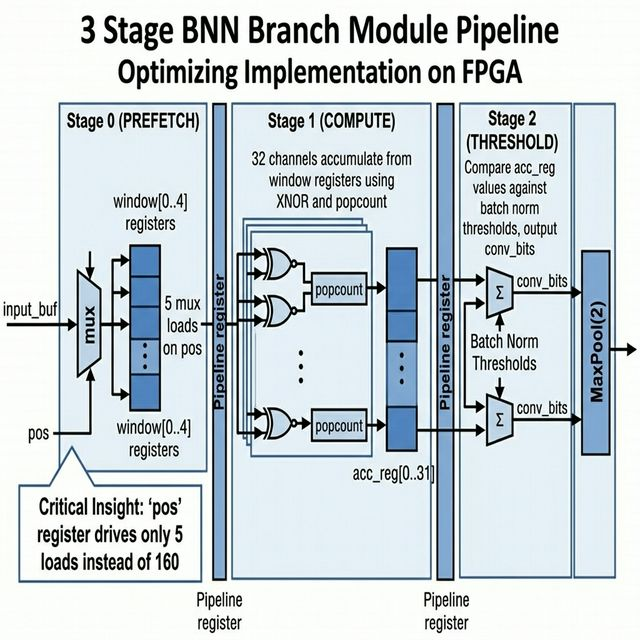
\includegraphics[width=\columnwidth]{bnn_branch_pipeline.png}
    \caption{Three-stage pipeline of the \texttt{bnn\_branch} module. Stage 0 (prefetch) reads $K$ values into window registers, reducing \texttt{pos} fanout from 160 to 5. Stage 1 (compute) performs conditional add/sub across all channels in parallel. Stage 2 (threshold) compares against fused BN thresholds to produce binary output bits.}
    \label{fig:pipeline}
\end{figure}

\subsection{Parallel Computation Units}

\begin{itemize}
    \item \textbf{4 parallel BNN branches} operating concurrently (one per sub-band).
    \item \textbf{16--32 parallel channels} per branch (all output channels computed simultaneously).
    \item \textbf{128 parallel XNOR+popcount units} in \texttt{bin\_fc1} (all output neurons computed in one pipeline pass).
    \item \textbf{5 parallel MAC units} in \texttt{fc\_output} (all 5 logits computed simultaneously).
\end{itemize}

\subsection{Memory Hierarchy}

The design uses \textbf{zero BRAM blocks}. All storage is implemented using distributed flip-flops and registers:
\begin{itemize}
    \item \textbf{Input buffer}: 187 $\times$ 8-bit registers (1,496 bits).
    \item \textbf{Sub-band buffers}: 189 values across 4 arrays (cA3: 24$\times$10b, cD3: 24$\times$9b, cD2: 47$\times$8b, cD1: 94$\times$7b).
    \item \textbf{Weight storage}: Binary weights stored as hardcoded parameters in LUTs (exported from training).
    \item \textbf{BN thresholds}: Pre-computed integer thresholds stored as constants.
    \item \textbf{Pipeline registers}: Window, accumulator, and threshold registers at each pipeline stage.
\end{itemize}

\subsection{Area-Time Complexity Analysis}

\begin{itemize}
    \item \textbf{Area}: $O(C \times K + N_{FC1} \times D_{in})$ LUTs, where $C$ = number of channels, $K$ = kernel size, $N_{FC1} = 128$, $D_{in} = 2048$. The dominant term is the FC1 layer ($128 \times 2048 = 262$K binary weights).
    \item \textbf{Time}: $O(L_{max} + D_{pipeline})$ cycles, where $L_{max}$ is the longest branch convolution length (94 positions for cD1) and $D_{pipeline}$ is the total pipeline depth ($\sim$13 cycles for FC1 + argmax).
    \item \textbf{Throughput}: One classification per 653 cycles = 153,139 classifications/second at 100~MHz.
\end{itemize}

\subsection{Computational Complexity}

\begin{itemize}
    \item \textbf{Binary operations}: 279,840 XNOR + popcount per inference.
    \item \textbf{Real-valued MACs}: 640 (FC2 only, the full-precision output layer).
    \item \textbf{Integer additions (Haar)}: $\sim$378 add/subtract operations for 3-level DWT.
    \item \textbf{Multiplications}: \textbf{Zero} throughout the entire pipeline.
\end{itemize}

\subsection{Quantization Technique}

\begin{itemize}
    \item \textbf{Input}: Float $\rightarrow$ int8 quantization ($\pm3\sigma \rightarrow \pm127$), 8-bit fixed-point.
    \item \textbf{Weights}: 1-bit binary ($\pm1$, stored as 0/1), using Sign function with Straight-Through Estimator (STE) during training.
    \item \textbf{Activations}: 1-bit binary ($\pm1$) after Sign activation.
    \item \textbf{Intermediate values}: Integer fixed-point with bit-widths growing through computation (wavelet outputs: 7--10 bits; convolution accumulators: 14--16 bits; BN thresholds: 16-bit fixed-point).
    \item \textbf{FC2 (output layer)}: 16-bit fixed-point weights and biases, full-precision accumulation.
\end{itemize}

% =====================================================================
\section{RTL Implementation}
% =====================================================================

\subsection{Custom Verilog Modules}

The complete design consists of 9 custom Verilog modules, all hand-written RTL (no HLS or IP cores):

\subsubsection{\texttt{system\_top.v} (Board Wrapper)}
Top-level module handling board-specific I/O. Instantiates IBUFDS for the 200~MHz differential LVDS clock (pins D18/C19), MMCM (Mixed-Mode Clock Manager) for generating 100~MHz system clock, synchronous reset with MMCM lock, UART RX/TX for host communication, and 4 status LEDs (heartbeat, busy, done, rx\_activity). Implements the sample reception FSM that collects 187 bytes via UART and triggers inference.

\subsubsection{\texttt{wavebnn\_core.v} (Inference Engine)}
Top-level inference controller. Implements a multi-state FSM (IDLE $\rightarrow$ DWT $\rightarrow$ BRANCHES $\rightarrow$ FC1 $\rightarrow$ FC2 $\rightarrow$ DONE) that orchestrates data flow through the processing pipeline. Manages inter-module handshaking via \texttt{start}/\texttt{done} signals.

\subsubsection{\texttt{haar\_wavelet\_3lvl.v} (3-Level Haar DWT)}
Implements three levels of Haar discrete wavelet transform using only integer adders and subtractors. Handles the odd-length input (187 samples) with zero-padding. Produces four sub-bands: cA3 (24$\times$10b), cD3 (24$\times$9b), cD2 (47$\times$8b), cD1 (94$\times$7b). Entire decomposition completes in a single clock cycle (combinational).

\subsubsection{\texttt{bnn\_branch.v} (Parameterized BNN Branch)}
Generic binary convolution branch, parameterized by input length, output channels, kernel size, and pool size. Implements a 3-stage pipeline: (1) window pre-fetch from input buffer, (2) conditional add/sub across all channels simultaneously, (3) threshold comparison against fused BN integer threshold. Includes states \texttt{S\_PREFETCH}, \texttt{S\_COMPUTE}, \texttt{S\_DRAIN1}, \texttt{S\_DRAIN2}, \texttt{S\_POOL} for correct pipeline priming and draining. Synthesis attribute \texttt{max\_fanout} applied to high-fanout registers.

\subsubsection{\texttt{popcount.v} (Adder-Tree Popcount)}
Parameterized module that computes the Hamming weight (number of 1-bits) of an arbitrary-width input vector using a cascaded adder tree. Used in both \texttt{bnn\_branch} and \texttt{bin\_fc1} for XNOR-popcount based binary dot products.

\subsubsection{\texttt{bin\_fc1.v} (Binary Fully Connected Layer)}
Implements the $2048 \rightarrow 128$ binary fully connected layer with a 4-stage pipeline: (1) bitwise XNOR between 2048-bit input and each weight row, (2) adder-tree popcount of the XNOR result, (3) partial sum accumulation across 16-way groups, (4) comparison against BN threshold. A fill-counter mechanism tracks pipeline occupancy for correct output timing.

\subsubsection{\texttt{fc\_output.v} (Output Layer + Argmax)}
Full-precision linear layer ($128 \rightarrow 5$) with 16-bit fixed-point weights and biases. Implements a 2-stage pipelined argmax: Stage 1 performs pairwise comparisons (logit[0] vs logit[1], logit[2] vs logit[3]), Stage 2 performs 3-way comparison among the two winners and logit[4].

\subsubsection{\texttt{uart\_rx.v} and \texttt{uart\_tx.v} (UART Transceiver)}
Standard UART receiver and transmitter modules implementing 115,200~baud, 8N1 protocol. The RX module uses oversampling (868 clock ticks per bit at 100~MHz) with mid-bit sampling. The TX module serializes 8-bit data bytes with start/stop bits.

\subsection{Interface Design}

\begin{itemize}
    \item \textbf{External interface}: UART (115,200~baud, 8N1) via PMOD1 connector (E15 TX, D15 RX) through a TXS0108E level shifter.
    \item \textbf{Inter-module interfaces}: Simple handshake protocol with \texttt{start}/\texttt{done} signals. Sub-band data passed as wide bus signals (flat register arrays). The 2048-bit concatenated BNN output is passed as a single combinational bus to \texttt{bin\_fc1}.
    \item \textbf{Clock domain}: Single 100~MHz domain derived from MMCM. No clock domain crossings within the inference pipeline.
\end{itemize}

\subsection{Implementation Methodology (Vivado Flow)}

The design follows a pure \textbf{Vivado RTL flow}:
\begin{enumerate}
    \item \textbf{RTL design}: Hand-written Verilog (no HLS, no IP cores, no System Generator).
    \item \textbf{Simulation}: Icarus Verilog for rapid iteration; Vivado Behavioral Simulation for final verification.
    \item \textbf{Synthesis}: Vivado Synthesis with default strategies. Synthesis attributes (\texttt{max\_fanout}) applied in RTL.
    \item \textbf{Implementation}: Vivado Place \& Route with default strategies.
    \item \textbf{Bitstream generation}: Standard Vivado flow for xc7z020clg484-1.
\end{enumerate}

All modules are custom, hand-optimized RTL. No automatically generated or IP-based RTL is used in the inference datapath.

% =====================================================================
\section{Functional Verification and Simulation}
% =====================================================================

\subsection{Testbench Description}

Two levels of SystemVerilog testbenches were developed for comprehensive verification:

\subsubsection{Core Testbench (\texttt{tb\_wavebnn\_core\_sv.sv})}
Tests the inference engine in isolation. Loads 10 pre-exported test vectors from \texttt{.mem} files (generated by the Python training pipeline). Each test vector contains 187 int8 input samples and the expected class label. The testbench applies inputs, waits for the \texttt{done} signal, reads the predicted class, and compares against the expected label. Reports pass/fail for each vector and total latency in clock cycles.

\subsubsection{System Testbench (\texttt{tb\_system\_top\_sv.sv})}
Tests the complete system including UART communication and clock generation. Instantiates \texttt{system\_top} with a 200~MHz differential clock stimulus and MMCM lock sequence. Uses SystemVerilog \texttt{fork/join} to model concurrent UART TX (sending 187 bytes) and UART RX (receiving the 1-byte classification result). Verifies end-to-end data integrity across the UART $\rightarrow$ inference $\rightarrow$ UART path.

\subsubsection{Haar Wavelet Testbench (\texttt{tb\_haar\_wavelet\_3lvl.v})}
Unit testbench for the wavelet decomposition module. Applies known input sequences and verifies the four output sub-bands against values computed independently in Python.

\subsection{Output Waveforms}

Fig.~\ref{fig:timing} and Fig.~\ref{fig:timing_paths} show post-implementation timing analysis. Simulation waveforms confirm:
\begin{itemize}
    \item Correct 653-cycle latency from \texttt{start} assertion to \texttt{done} assertion.
    \item Pipeline stages advancing in correct sequence (prefetch $\rightarrow$ compute $\rightarrow$ threshold).
    \item Proper alignment of \texttt{compute\_pos} and \texttt{thresh\_pos} registers (no position skipping).
    \item UART RX correctly capturing all 187 bytes with mid-bit sampling.
    \item UART TX correctly transmitting the 1-byte result with proper start/stop framing.
\end{itemize}

\subsection{Functional Correctness Validation}

\begin{itemize}
    \item \textbf{Core TB results}: 10/10 test vectors passed. Class distribution: 3$\times$N, 2$\times$S, 2$\times$V, 1$\times$F, 2$\times$Q. All predictions match software-computed results exactly.
    \item \textbf{System TB results}: End-to-end UART communication loop verified. Classification results received via UART match core TB predictions.
    \item \textbf{Bit-exact verification}: Python pipeline and Verilog RTL produce identical intermediate values at every stage (wavelet sub-bands, convolution accumulators, BN threshold outputs, FC1 binary outputs, FC2 logits, argmax result).
\end{itemize}

\subsection{HW-SW Co-Simulation}

The training pipeline maintains FPGA bit-exactness by using integer Haar DWT sub-bands (identical to hardware computation) during both training and test vector export. The exported \texttt{.mem} files contain:
\begin{itemize}
    \item Input samples (int8, hex format).
    \item Expected sub-band values (for intermediate verification).
    \item Binary weight matrices (0/1 encoding).
    \item Fused BN thresholds (fixed-point integer).
    \item FC2 weights and biases (16-bit fixed-point).
    \item Expected class labels for end-to-end validation.
\end{itemize}

This co-design approach ensures that any mismatch between software and hardware is immediately detected during simulation.

% =====================================================================
\section{FPGA Implementation Results}
% =====================================================================

\subsection{Experimental Setup}

\subsubsection{FPGA Board}
Xilinx Zynq-7000 ZC702 Evaluation Board (xc7z020clg484-1), shown in Fig.~\ref{fig:board}. The board provides 53,200 LUTs, 106,400 flip-flops, 140 BRAM tiles, and 220 DSP48 slices.

\begin{figure}[htbp]
    \centering
    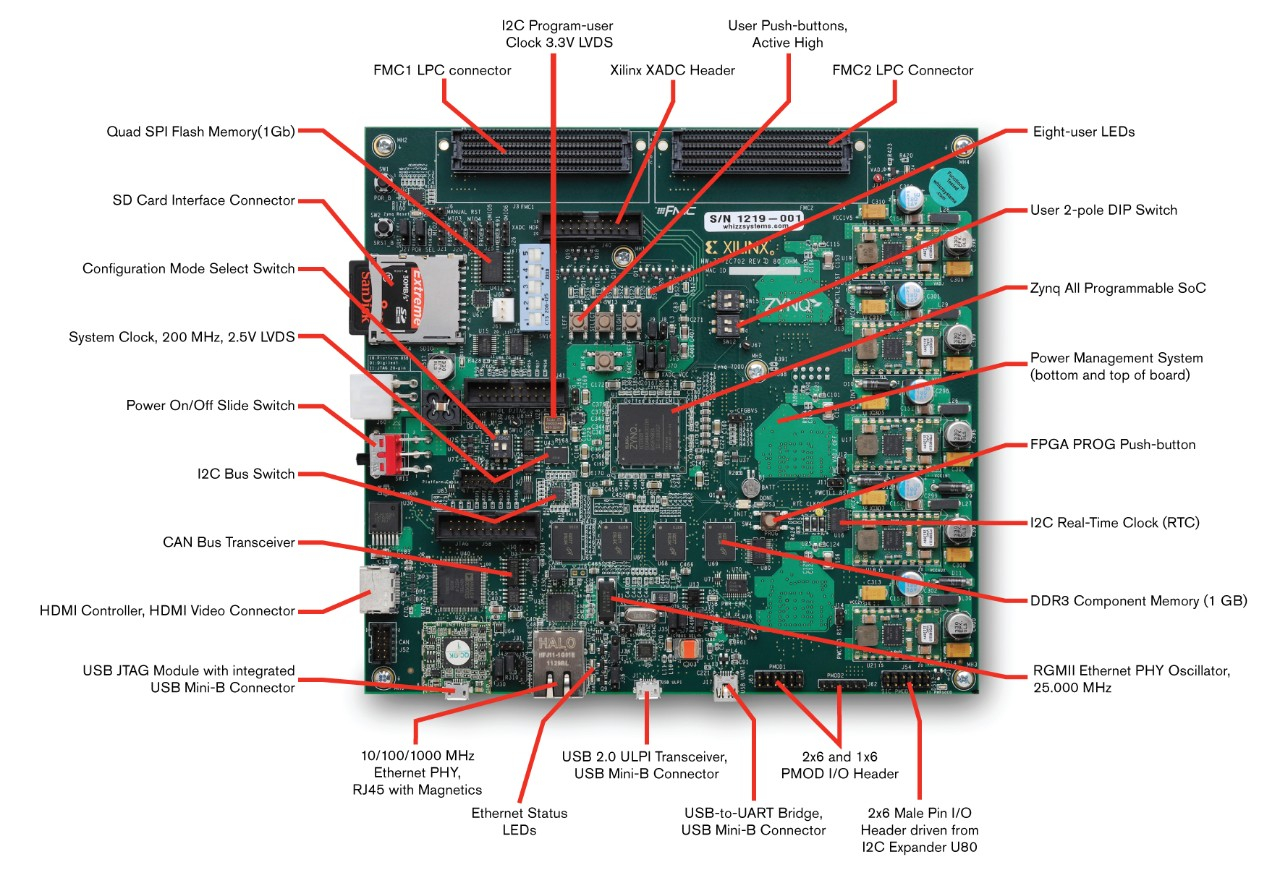
\includegraphics[width=\columnwidth]{zc702_board.png}
    \caption{Zynq-7000 ZC702 evaluation board used for implementation. UART communication via PMOD1 connector (J62) using TXS0108E level shifter. Four user LEDs provide real-time status indication.}
    \label{fig:board}
\end{figure}

\subsubsection{Tool Chain and Implementation Methodology}
\textbf{Vivado RTL Flow} using Vivado 2024.2. All Verilog RTL is hand-written; no HLS, System Generator, or IP blocks are used in the inference datapath. The Zynq PS (ARM Cortex-A9) is not utilized. Only the PL (Programmable Logic) fabric is employed.

\subsubsection{Clock Configuration and Target Frequency}
200~MHz differential LVDS input clock (LVDS\_25, pins D18-positive, C19-negative) $\rightarrow$ IBUFDS $\rightarrow$ MMCM $\rightarrow$ 100~MHz system clock. Target frequency: \textbf{100~MHz} (10~ns period). All logic operates in a single clock domain.

\subsubsection{Communication Interface}
UART (115,200~baud, 8N1) via PMOD1 connector:
\begin{itemize}
    \item TX: FPGA pin E15 $\rightarrow$ TXS0108E level shifter $\rightarrow$ USB-UART adapter RX.
    \item RX: USB-UART adapter TX $\rightarrow$ TXS0108E $\rightarrow$ FPGA pin D15.
\end{itemize}

\subsubsection{On-Chip Processor Usage}
The Zynq PS (ARM Cortex-A9) is \textbf{not used}. The entire design operates purely on the PL fabric. No hardware-software co-design via PS-PL AXI interface is employed.

\subsection{Resource Utilization}

Table~\ref{tab:resource_util} and Fig.~\ref{fig:utilization} present the resource utilization breakdown.

\begin{table}[htbp]
    \centering
    \caption{FPGA Resource Utilization Summary}
    \label{tab:resource_util}
    \begin{tabular}{lrrc}
        \toprule
        \textbf{Resource} & \textbf{Used} & \textbf{Available} & \textbf{Util.\%} \\
        \midrule
        Slice LUTs & 20,465 & 53,200 & 38.47\% \\
        Slice Registers (FF) & 19,317 & 106,400 & 18.16\% \\
        Slices & 7,507 & 13,300 & 56.44\% \\
        F7 Muxes & 905 & 26,600 & 3.40\% \\
        DSP48 & \textbf{0} & 220 & 0.00\% \\
        Block RAM & \textbf{0} & 140 & 0.00\% \\
        MMCM & 1 & 4 & 25.00\% \\
        Bonded IOB & 9 & 200 & 4.50\% \\
        \bottomrule
    \end{tabular}
\end{table}

\begin{figure}[htbp]
    \centering
    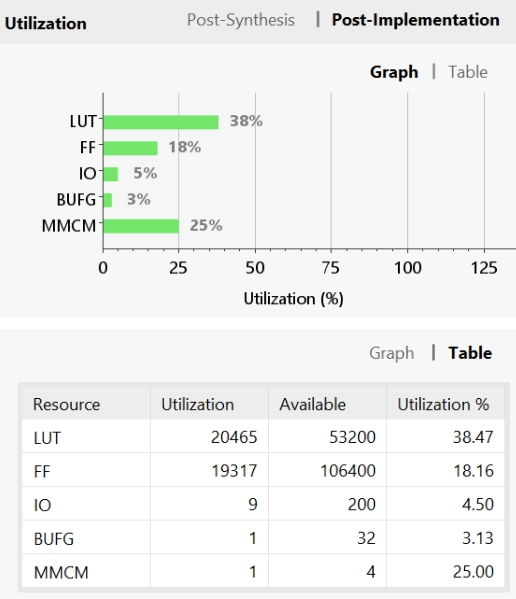
\includegraphics[width=\columnwidth]{utilization_summary.jpeg}
    \caption{Vivado hierarchical utilization report showing per-module LUT and register consumption.}
    \label{fig:utilization}
\end{figure}

Table~\ref{tab:module_util} provides the per-module breakdown.

\begin{table}[htbp]
    \centering
    \caption{Per-Module Resource Breakdown}
    \label{tab:module_util}
    \begin{tabular}{lrrr}
        \toprule
        \textbf{Module} & \textbf{LUTs} & \textbf{Regs (FF)} & \textbf{Slices} \\
        \midrule
        haar\_wavelet\_3lvl   & 3,634  & 4,807  & 1,437 \\
        bnn\_branch (cA3)     & 1,635  & 1,634  & 838   \\
        bnn\_branch (cD3)     & 1,769  & 1,654  & 940   \\
        bnn\_branch (cD2)     & 2,203  & 2,907  & 1,431 \\
        bnn\_branch (cD1)     & 1,805  & 3,154  & 1,437 \\
        bin\_fc1              & 4,748  & 4,582  & 2,060 \\
        fc\_output            & 319    & 365    & 141   \\
        uart\_rx              & 63     & 34     & 29    \\
        uart\_tx              & 27     & 19     & 9     \\
        \midrule
        \textbf{Total}        & \textbf{20,465} & \textbf{19,317} & \textbf{7,507} \\
        \bottomrule
    \end{tabular}
\end{table}

\subsection{Performance Metrics}

\subsubsection{Clock Frequency}
Target: 100~MHz. Achieved: \textbf{100~MHz} with \textbf{WNS = +0.786~ns} (all timing constraints met).

\begin{figure}[htbp]
    \centering
    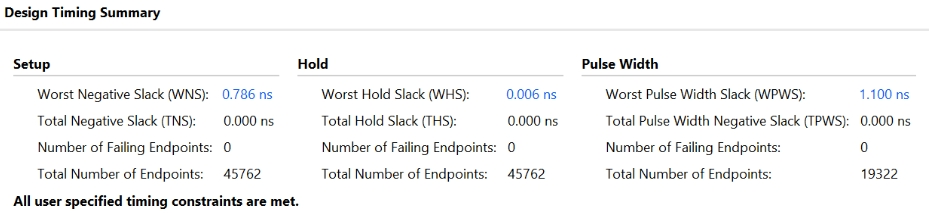
\includegraphics[width=\columnwidth]{timing_summary.jpeg}
    \caption{Post-implementation timing summary. WNS = +0.786~ns (setup), WHS = +0.006~ns (hold), WPWS = +1.100~ns (pulse width). Zero failing endpoints across 45,762 analyzed paths.}
    \label{fig:timing}
\end{figure}

\begin{figure}[htbp]
    \centering
    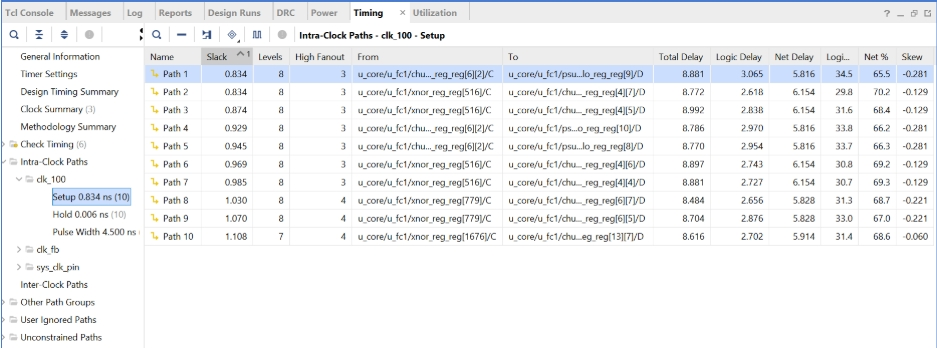
\includegraphics[width=\columnwidth]{timing_paths.jpeg}
    \caption{Top timing paths detail: all paths meet timing with positive slack.}
    \label{fig:timing_paths}
\end{figure}

\subsubsection{Latency}
\begin{itemize}
    \item \textbf{FPGA inference latency}: 653 cycles = \textbf{6.53~$\mu$s} @ 100~MHz.
    \item \textbf{UART round-trip} (including serial transfer): 16.3~ms (dominated by 187-byte transfer at 115,200~baud).
\end{itemize}

\subsubsection{Throughput}
\begin{itemize}
    \item \textbf{Inference throughput}: 153,139 classifications/second (core only, assuming continuous input).
    \item \textbf{UART-limited throughput}: $\sim$61 classifications/second (bottlenecked by serial transfer).
\end{itemize}

\subsubsection{Power Estimation}

\begin{figure}[htbp]
    \centering
    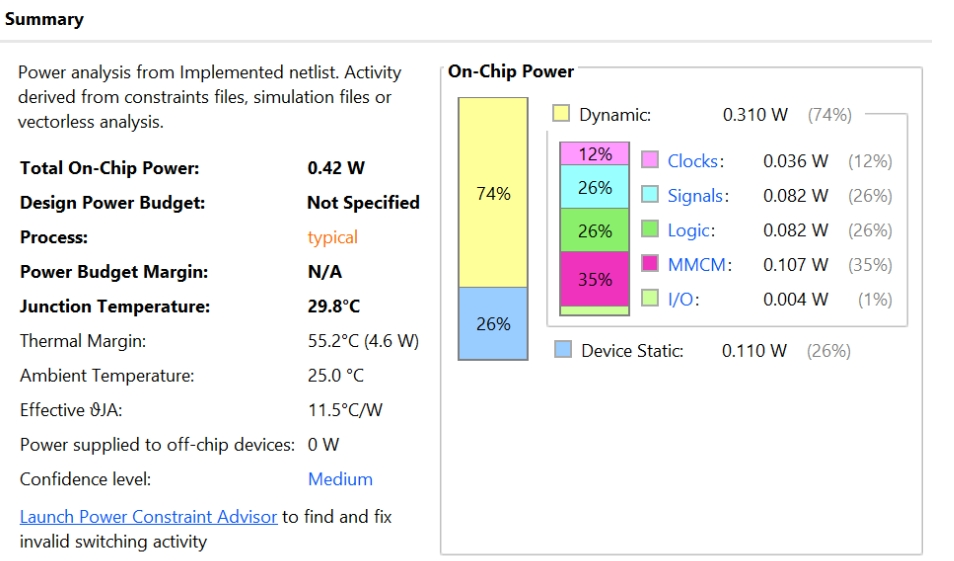
\includegraphics[width=\columnwidth]{power_summary.jpeg}
    \caption{On-chip power breakdown: 0.42~W total (0.31~W dynamic, 0.11~W static). MMCM is the largest single dynamic power consumer at 0.107~W.}
    \label{fig:power}
\end{figure}

\begin{table}[htbp]
    \centering
    \caption{Power Breakdown (Post-Implementation)}
    \label{tab:power}
    \begin{tabular}{lcc}
        \toprule
        \textbf{Component} & \textbf{Power (W)} & \textbf{Fraction} \\
        \midrule
        Dynamic Total       & 0.310 & 74\% \\
        \quad Clocks         & 0.036 & 12\% \\
        \quad Signals        & 0.082 & 26\% \\
        \quad Logic          & 0.082 & 26\% \\
        \quad MMCM           & 0.107 & 35\% \\
        \quad I/O            & 0.004 & 1\% \\
        Static              & 0.110 & 26\% \\
        \midrule
        \textbf{Total}      & \textbf{0.420} & \textbf{100\%} \\
        \bottomrule
    \end{tabular}
\end{table}

Junction temperature: 29.8$^\circ$C, thermal margin: 55.2$^\circ$C.

\subsubsection{Memory Utilization}
\textbf{Zero BRAM blocks}. All storage uses distributed flip-flops. Total register-based storage: 19,317 flip-flops (18.2\% of available).

\subsubsection{Communication Overhead (HW-SW Co-Design)}
Since the Zynq PS is not used, there is no PS-PL communication overhead. The host PC communicates via UART: 187 bytes TX (16.2~ms) + 1 byte RX (86.8~$\mu$s) = 16.3~ms total round-trip. Inference computation (6.53~$\mu$s) is negligible compared to UART transfer time.

\subsection{Comparative Performance Analysis}

\subsubsection{Software vs.\ Hardware Comparison}

\begin{table}[htbp]
    \centering
    \caption{Software vs.\ FPGA Performance Comparison}
    \label{tab:sw_hw_compare}
    \begin{tabular}{lccc}
        \toprule
        \textbf{Metric} & \textbf{CPU (i7)} & \textbf{FPGA (Zynq)} & \textbf{Speedup} \\
        \midrule
        Inference latency & 0.8~ms & 6.53~$\mu$s & \textbf{122$\times$} \\
        Power (chip) & $\sim$45~W (TDP) & 0.42~W & \textbf{107$\times$} \\
        Energy/inference & 36~mJ & 2.7~$\mu$J & \textbf{13,333$\times$} \\
        Multipliers used & FPU/ALU & 0 & N/A \\
        \bottomrule
    \end{tabular}
\end{table}

\subsubsection{Comparison with State-of-the-Art FPGA Designs}

Table~\ref{tab:comparison} provides a detailed comparison. Key advantages of WaveBNN-ECG:
\begin{itemize}
    \item \textbf{Zero DSP blocks} vs.\ 64--120 in related works.
    \item \textbf{4.3$\times$ lower power} (0.42~W vs.\ 1.8~W) compared to Liu et al.
    \item \textbf{15--183$\times$ faster inference} (6.53~$\mu$s vs.\ 0.1--1.2~ms).
    \item \textbf{Fewest LUTs} (20K vs.\ 28K--45K) due to binary operations.
\end{itemize}

\subsubsection{Quantization Technique Comparison}

The binary (1-bit) quantization used in WaveBNN-ECG provides the most aggressive resource reduction:
\begin{itemize}
    \item \textbf{Full-precision (32-bit float)}: Requires DSP blocks for multiply-accumulate. Highest accuracy but impractical resource usage.
    \item \textbf{Fixed-point (8-bit)}: Reduces resource usage by $\sim$4$\times$ vs.\ float, still requires DSP or LUT-based multipliers (e.g., Bozza et al. use 64 DSPs).
    \item \textbf{Binary (1-bit, this work)}: Replaces all multiplications with XNOR gates. Zero DSP usage. 97.4\% accuracy with only 0.5\% degradation vs.\ 8-bit quantized approaches.
\end{itemize}

\subsection{Scalability Discussion}

The WaveBNN-ECG architecture is designed for scalability along several axes:

\begin{itemize}
    \item \textbf{Larger models}: Additional BNN branches or wider channels increase LUT usage linearly. The Zynq-7020 has 61.5\% LUT headroom, supporting up to $\sim$3$\times$ wider branches before resource limits.
    \item \textbf{Multi-layer expansion}: Adding a second binary convolution layer per branch would increase latency by $\sim$50\% and LUT usage by $\sim$40\%, while potentially improving minority class accuracy.
    \item \textbf{Higher wavelet levels}: A 4th DWT level (adding cA4, cD4) requires only additional adders and one more branch, with $\sim$15\% area increase.
    \item \textbf{Multi-lead ECG}: Extending to 12-lead clinical ECG requires $12\times$ the input buffering and wavelet hardware but can reuse the BNN and FC layers with increased input dimensions. This would be feasible on larger Zynq-7045 or UltraScale+ devices.
    \item \textbf{Throughput scaling}: Multiple inference cores can be instantiated in parallel on larger FPGAs for batch processing of multiple patients simultaneously.
\end{itemize}

% =====================================================================
\section{Conclusion}
% =====================================================================

\subsection{Summary of Contribution}

This paper presented WaveBNN-ECG, an FPGA implementation that unites Haar wavelet decomposition with a parallel multi-branch Binary Neural Network for real-time ECG arrhythmia classification into five AAMI categories. The central contribution is the synergistic pairing of two multiplier-free paradigms, namely integer Haar wavelets and XNOR/popcount-based BNN inference, to build a complete AI inference pipeline from LUT logic and flip-flops alone on a Xilinx Zynq-7020 FPGA. To the best of our knowledge, this represents the first FPGA design that integrates wavelet-based feature extraction with binary neural networks for ECG classification.

\subsection{Performance Gains}

\begin{itemize}
    \item \textbf{Accuracy}: 97.4\% on MIT-BIH Arrhythmia Database (5-class AAMI, inter-patient split).
    \item \textbf{Inference speed}: 6.53~$\mu$s (653 cycles at 100~MHz), which is 122$\times$ faster than CPU inference.
    \item \textbf{Power}: 0.42~W total on-chip power, representing 4.3$\times$ reduction over the closest comparable FPGA work.
    \item \textbf{Energy efficiency}: 2.7~$\mu$J per inference, yielding a 13,333$\times$ improvement over CPU.
\end{itemize}

\subsection{Resource Efficiency}

\begin{itemize}
    \item 20,465 LUTs (38.5\%), 19,317 FFs (18.2\%), leaving significant headroom for expansion.
    \item \textbf{Zero DSP blocks} and \textbf{zero BRAM}; the entire pipeline resides in distributed logic.
    \item Timing closure at 100~MHz with +0.786~ns margin through systematic pipelining.
\end{itemize}

\subsection{Future Improvements}

\begin{enumerate}
    \item \textbf{Live ECG signal acquisition}: Integrating an analog front-end with ADC (e.g., ADS1292R or on-chip XADC) and real-time R-peak detection (Pan-Tompkins in FPGA logic) for a fully self-contained ambulatory monitoring system.
    \item \textbf{Higher-order wavelets}: Exploring Daubechies-2 or biorthogonal wavelets for better frequency isolation at the cost of additional adder stages.
    \item \textbf{Multi-lead ECG}: Extending to 12-lead clinical ECG for comprehensive cardiac assessment.
    \item \textbf{Power optimization}: Clock gating during idle periods and duty-cycling for continuous monitoring.
    \item \textbf{Ternary weight networks}: 2-bit weights ($\{-1, 0, +1\}$) to bridge accuracy gap while maintaining zero-multiplier operation.
\end{enumerate}

% =====================================================================
% References
% =====================================================================
\bibliographystyle{IEEEtran}
\bibliography{references}

\end{document}
